\section{Theorie}
Dreht sich ein Körper der Masse m um eine Drehachse durch seinen Schwerpunkt, so wirkt auf diesen Körper das Drehmoment M mit
\begin{equation}
\vec{M} = \vec{F} \times \vec{r}.
\end{equation}

Ebenso wirkt ein Trägheitsmoment I, das bei mehreren Masseelementen $m_i$ mit 
\begin{equation}
I = \sum_{i} {r_i}^2 \cdot m_i
\end{equation}
gegeben ist, wobei $r_i$ der Abstand der rotierenden punktförmigen Massen $m_i$ zur Drehachse durch den Massenschwerpunkt ist.
Für das Trägheitsmoment bei infinitisimalen Massen dm gilt
\begin{equation}
I = \int {r_i}^2 \, \symup{d}m.
\end{equation}

Mithilfe des Steinerschen Satzes kann das Trägheitsmoment eines Körpers der Masse m berechnet werden, wenn die Drehachse nicht durch 
den Massenschwerpunkt geht, sondern parallel um einen Abstand a verschoben ist:
\begin{equation}
I = I_s + m \cdot a^2.
\end{equation}
Hierbei ist $I_s$ das Trägheitsmoment des Körpers bei der Drehung um die Drehachse durch den Schwerpunkt.

Bei dem durchgeführten Versuch wurden Körper um einen Winkel $\varphi$ ausgelenkt. Beim Loslassen wirkt das Drehmoment M dann als
rücktreibende Kraft. Damit führt der Körper eine harmonische Schwingung mit einer Periodendauer T aus, wobei T mithilfe des
Trägheitsmoments I und der Winkelrichtgröße D über
\begin{equation}
T = 2\pi \sqrt{\frac{I}{D}}
\label{eqn:periodendauer}
\end{equation}
berechnet werden kann.   
Bei der statischen Methode kann bei bekanntem Drehmoment die Winkelrichtgröße D entweder über den Zusammenhang
\begin{equation}
M = D \cdot \varphi 
\end{equation}
bestimmt werden oder bei der dynamische Methode durch Messung der Periodendauer und Bestimmung des Trägheitsmoments mit 
Gleichung \eqref{eqn:periodendauer}.
Die Formel für die Trägheitsmomente verschiedener Körper sind in Abbildung \ref{fig:abb2} zu finden.
\begin{figure}
\centering
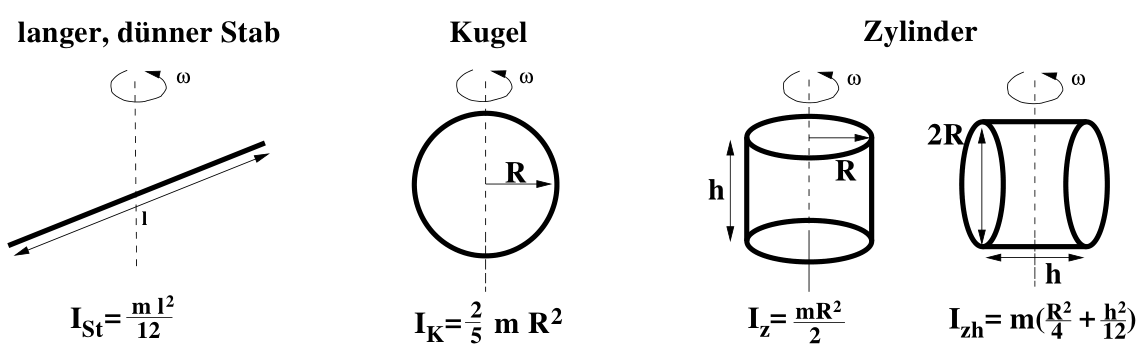
\includegraphics[scale=.5]{Traegheitsmomente101.png}
\caption{Trägheitsmomente verschiedener Körper.\cite[1]{anleitung101}}
\end{figure}


